\begin{Problem}
	Wir definieren mit $S_n$ die Menge der bijektiven Abbildungen
	\[
	\sigma:\left\{ 1,\dots,n \right\} \to \left\{ 1,\dots,n \right\} 
	.\] 
	Dann ist bekannterweise $(S,\circ)$ mit
	\[
	\sigma_2\circ \sigma_1(i)=\sigma_2(\sigma_1(i))
	\]
	eine Gruppe. Wir führen für gewöhnlich eine Abbildungstabelle
	\[
		\sigma=\begin{pmatrix} 1 & 2 & \dots & n \\ i_1 & i_2 & \dots & i_n \end{pmatrix} \] 
		mit $i_1,\dots,i_n$ paarweise verschieden, um zu signalisieren $\sigma(k)=i_k$ f\"{u}r $k=1,\dots,n$.
		 \begin{parts}
			 \item Eine übliche Darstellung bei Elementen aus $S_n$ ist die Zyklenschreibweise. Ein Zyklus der Länge $k$ mit $k\le n$ hat die Form
				 \[
				 \sigma=(i_1,i_2,\dots, i_k)
				 \]
				 und signalisiert $i_1\to i_2, i_2\to i_3$, usw. $i_k\to i_1$ under $\sigma$. Ist die Zahl $i_j$ nicht im Zyklus vertreten, so wird sie unter $\sigma$ auf sich selbst abgebildet. Speziell f\"{u}r $k=1$ erhalten wir die Identität und schreiben
				 \[
				 \sigma=(1).\]
Geben Sie an, wie viele unterschiedliche Abbildungen $\sigma$ durch ein Zyklus der Länge $k$ realisiert werden können! Kann jedes Element in $S_3$ ($S_4$) als ein Zyklus geschriebeb werden?
\item Wir definieren die Menge der (Permutations-)Matrizen
	\[
		P_n:=\left\{ P\in \mathbb{K}^{n \times  n}: P=(e_{i_1},\dots,e_{i_n},\text{ mit }i\le i_k\le n\text{ und alle }i_k\text{ paarweise verschieden} \right\} 
	,\] 
	mit $e_i$ der $i$-te Einheitsvektor. Verifizieren Sie: $(P_n, \cdot)$ ist mit der herkömmlichen Matrixmultiplikation eine Gruppe! Bestimmen Sie weiterhin einen bijektiven Gruppenmorphismus
	\[
	\Phi:(S_n,\circ)\to(P_n,\cdot)
	,\] 
	sodass gilt
	\[
	\Phi(\sigma)e_i=s_j \iff\sigma(i)=j
	.\] 
	Beweisen Sie, dass sich jedes $P$ aus $P_n$ schreiben lässt als
	\[
		P=\prod_{k=1}^{n-1} V_{i_kj_k} 
	,\]
	mit $V_{ij}$ definiert wie in Lemma 5.56.
		\end{parts}
\end{Problem}
\begin{proof}
	\begin{parts}
	\item Es gibt $n!$ Möglichkeiten f\"{u}r eine Folge $(i_1i_2\dots i_k)$, aber wir können die zyklisch permutieren und $\sigma$ verändert sich nicht. Deswegen gibt es $n! / n = (n-1)!$ unterschiedliche Abbildungen, die durch ein Zyklus der Länge $k$ realisiert werden können.

		Ja, jedes Element in $S_3$ kann als ein Zyklus geschrieben werden. Das können wir explizit machen:
		\begin{align*}
			& (1) & (12) & & (23)\\
			& (13) & (132) & & (123)
		\end{align*}
		Weil wir $6$ Elemente haben, und $|S_3|=3! = 6$, haben wir alle Elemente.

		Das stimmt aber nicht f\"{u}r $S_4$. Sei
		\[
			\sigma=\begin{pmatrix} 1 & 2 & 3 & 4\\ 2 & 1 & 4 & 3 \end{pmatrix} 
		.\] 
		Falls es als Zyklus geschreiben werden kann, muss das Zyklus den Länge $4$ haben, weil $\sigma(i)\neq i$ f\"{u}r alle $i$. Wir fangen obdA mit $1$ an. Dann ist das Zyklus $(12\dots)$. Aber weil $\sigma(2)=1$, hört das Zyklus auf, und $\dots=\varnothing$. Dann ist das Zyklus nicht mit Länge 4. 
	\item Sei $A,B\in P_n$ beliebige Elemente von $P_n$,
		\begin{align*}
			A=&(e_{i_1},e_{i_2},\dots, e_{i_n})\\
			B=&(e_{j_1},e_{j_2},\dots, e_{j_n})
		\end{align*}
		\begin{enumerate}[label=(\roman*)]
			\item $G$ ist abgeschlossen: Wir betrachten $ABe_k$ f\"{u}r $k$ beliebig.
				\[
					ABe_k=Ae_{j_k}=e_{i_{j_k}}
				,\]
				also
				\[
					AB=(e_{i_{j_1}},e_{i_{j_2}},\dots,e_{i_{j_n}})\in P_n
				.\] 
				Das $i_{j_k}$ paarweise verscheiden sind folgt daraus, dass $j_k$ alle paarweise verscheiden sind.
			\item Neutrales element: Wir wissen aus der linearen ALgebra, dass
				 \[
				1_n=(e_1,e_2,\dots, e_n)\in P_n
				\]
				das neutrales Element ist.
			\item Assoziativität: Wir wissen auch, dass Matrizmultiplikation assoziativ ist.
			\item Existenz des Inverses: Sei jetzt $p_k$, sodass $i_{p_k}=k$. 
				\begin{tcolorbox}[title=Bemerkung]
					Man kann $i,p: \left\{ 1,\dots,n \right\} \to \left\{ 1,\dots,n \right\} $ interpretieren. Dann ist $i$ eine bijektive Abbildung, und das Existenz einer inversen Abbildung $p$ folgt daraus. Deswegen ist unsere Entscheidung immer möglich.
				\end{tcolorbox}
				Wir betrachten $A(e_{p_1},e_{p_2},\dots, e_{p_n})$, und dafür die Wirkung der Abbildung auf einem beliebigen Basiselement $e_k$: 
\[
	A(e_{p_1},e_{p_2},\dots,e_{p_n})e_k=Ae_{p_k}=e_{i_{p_k}}=e_k
.\] 
		\end{enumerate}
	\item Sei $i$ eine bijektive Abbildung $\left\{ 1,\dots,n \right\}\to \left\{ 1,\dots,n \right\} $. Wir schreiben $i_k$ oder $i(k)$ als das Bild von $k$. Wir vermuten, dass die gewünschte Homomorphismus
		\[
		\Phi:i\to (e_{i_1},e_{i_2},\dots e_{i_n})
		\] 
		ist.
		\begin{enumerate}[label=(\roman*)]
			\item $\Phi(\sigma)e_j=e_{\sigma_j}$, also  $\Phi(\sigma)e_i=s_j\iff \sigma(i)=j$.
			\item Injektiv: Sei $\sigma,\sigma' \in S_n$, $\sigma\neq \sigma'$, insbesondere gilt $\sigma(i)\neq \sigma'(i)$. Es gilt dann
				 \begin{center}
					 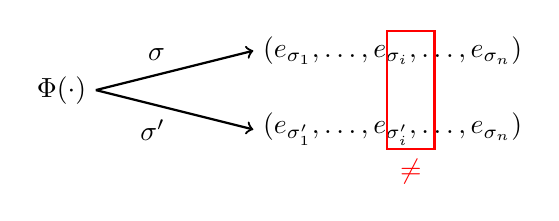
\begin{tikzpicture}[xscale=2,yscale=0.5]
						\draw (0,0) node[anchor=east] {$\Phi(\cdot)$};
						\draw[thick,->] (0,0) -- (1,1);
						\draw[thick,->] (0,0) -- (1,-1);
						\draw (1,1) node[anchor=west] {$(e_{\sigma_1},\dots,e_{\sigma_i},\dots,e_{\sigma_n})$};
						\draw (1,-1) node[anchor=west] {$(e_{\sigma'_1},\dots, e_{\sigma'_i},\dots,e_{\sigma_n})$};
						\draw (0.5,0.5) node[anchor=south east] {$\sigma$};
						\draw (0.5,-0.5) node[anchor=north east] {$\sigma'$};
						\draw[red,thick] (1.85,-1.5) rectangle (2.15,1.5);
						\draw[red] (2,-1.5) node[anchor=north] {$\neq$};
					\end{tikzpicture}
				\end{center}
				also $\Phi(\sigma)\neq \Phi(\sigma')$.
			\item Surjektiv: Sei $M=(e_{i_1},e_{i_2},\dots,e_{i_n}$. Wie im letzten Teilaufgabe können wir eine Abbildung $i(k)=i_k$ definieren, und $\Phi(i)=M$.
			\item Homomorphismusgesetz: Es ist zu zeigen, f\"{u}r $i,j\in S_n$ und 
				\begin{align*}
					M_1=&(e_{i_1},e_{i_2},\dots, e_{i_n})=\Phi(i)\\
					M_2=&(e_{j_1},e_{j_2},\dots,e_{j_n})=\Phi(j),
				\end{align*}
				dass
				 \[
				\Phi(i \circ j)(e_k)=M_1M_2e_k
				\] 
				f\"{u}r alle $k$ gilt. Per Definition ist
				\[
					\Phi(i\circ j)e_k=e_{i(j(k))}=e_{i_{j_k}}
				.\] 
				Es gilt auch
				\[
					M_1M_2e_k=M_1e_{j(k)}=e_{i(j(k))}=e_{i_{j_k}}
				.\] 
		\end{enumerate}
	\end{parts}
\end{proof}
\begin{Problem}
	Gegeben sei die Permutation
	\[
		S_9\ni \sigma =\begin{pmatrix} 1 & 2 & 3 & 4 & 5 & 6 & 7 & 8 & 9\\2 & 4 & 3 & 9 & 7 & 6 & 8 & 1 & 5 \end{pmatrix} 
	.\] 
	\begin{parts}
	\item Stellen sie $\sigma$ als Produkt von Transpositionen dar.
	\item Berechnen Sie das Signum von $\sigma$.
	\end{parts}
\end{Problem}
